\chapter{Parallel Metropolis-Hastings}
In the chapter above, the fundamental Metropolis-Hastings were implemented and evaluated. In this chapter, we modify the fundamental Metropolis-Hastings algorithm, so that it can be run in a parallel way to optimize the run time.

\section{General Idea of Parallel Metropolis-Hastings}
In fundamental Metropolis-Hastings, we use a Markov chain to generate new samples. However, it would be possible to fully exploit the parallel computing property and run the algorithm with multiple Markov chains. The general idea would be to use multiple Markov chains instead of one single chain to generate samples. For instance, instead of drawing 10000 samples from one single Markov chain, we draw 2000 samples from five Markov chains simultaneously. 

This modification leads to several aspects that should be discussed. For one, the combination of all of the samples could give rise to some problems. Since the Markov chain will eventually generate a sample from a given stationary distribution, all the samples generated across different chains will be sampled from the same stationary distribution. Therefore, we can simply combine the results after the burn-in period that are derived from different chains. Nevertheless, we need to make sure that all the samples that are generated from the chain after the burn-in period need to be sampled from the stationary distribution. Since each Markov chain from the parallel Metropolis-Hastings generates fewer samples than the amounts of samples that are generated by the Markov chain in the fundamental algorithm, it might be the case that some of the Markov chains do not reach the point where they sample from the stationary distribution. To examine this, we can use the trace plot~\cite{mcmc_practice}. It will be discussed in the section "Trace Plot" in this chapter.

Another problem would be the convergence of each dimension. After obtaining the final results, we need to make sure that each dimension of the Bayesian inferred result needs to deliver a converged result, which means that the entire result after the combination is stable and representative and reaches a stationary distribution. In a later section called "Gelman Rubin Convergence", we use the metric of Gelman Rubin Convergence to examine whether the Bayesian inferred result for the hydrological model using the parallel Metropolis-Hastings reaches convergence.

\section{Efficiency Analysis}
Since the machine, on which the algorithm is run, has 10 cores of CPUs, we are going to experiment with this algorithm with 10, 8, 5, 4, and 2 chains. These cases will be compared with the fundamental Metropolis-Hastings algorithm, where only one single chain is run. To analyze the algorithm concerning its efficiency, we record the run time of the algorithm using different numbers of chains. The result is represented in Figure 5.1. It is obvious to see that the run time and the number of chains display an inverse proportional relationship. The more chains that are used, the less time is required for the algorithm to run, and vice versa.

\begin{figure}[H]
    \centering
    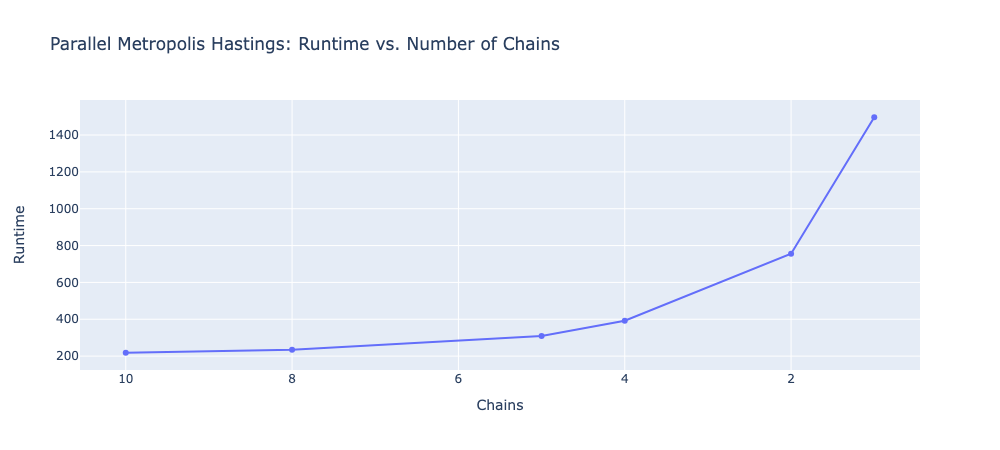
\includegraphics[width=1\textwidth]{figures/parallel_mh/runtime.png}
    \captionsetup{width=.8\textwidth}
    \caption{Relationship between run time and chain numbers for parallel Metropolis-Hastings algorithm}
    \label{fig:enter-label}
\end{figure}

\section{Trace Plot}
Making sure that each Markov chain generates samples from the stationary distribution is crucial in the parallel Metropolis-Hastings algorithm. The best way to examine this aspect is to visualize the trace of each sample generated from the chain~\cite{mcmc_practice}. The trace plot tracks each sample generated by the algorithm and plots the position of each sample by order. In this case, we can observe which sample is generated based on the last sample.

As mentioned before, it is more likely that the parallel Metropolis-Hastings algorithm with more chains shows less probability of sampling from stationary distribution than the parallel Metropolis-Hastings algorithm with fewer chains. This aspect is going to be analyzed now. We first select random chains from the algorithm run with the most number of chains, namely $10$, and the least number of chains, which is $2$, to observe the two extreme cases. Since 1000 samples are generated by each chain from the case of $10$ chains, only $266$ samples are going to be recorded after discarding $20\%$ of the burn-in and using $3$ as the effective sample size. With the case of $2$ chains, the number of samples recorded has risen to $1333$, which is almost $5$ times as much as the previous case. This shows a higher probability that the samples are generated from the stationary distribution.

For both cases, two chains are selected for visualization to ensure the generality of the analysis. The figures of the trace plots are displayed in Figures 5.2 to 5.5. One major difference between the visualizations of both cases is that the chain for case $10$ includes more abrupt jumps throughout the entire sampling process, whereas abrupt jumps occur less after the starting period is over for case $2$. The longer chain in the case of $2$ generally provides better stability and convergence of the parameter estimates. With no obvious sampling trends and full exploration of the entire parameter space, it is observable that every parameter for the chain has settled into a stationary distribution that covers the entire parameter space. The shorter chain in the case of $10$ may not enter the convergence and can be more susceptible to initial conditions or random fluctuations. Therefore, observing the trace plot for each chain after executing the algorithm is important, especially for algorithms that are run with more chains, each of which generates fewer samples.

\begin{figure}[H]
    \centering
    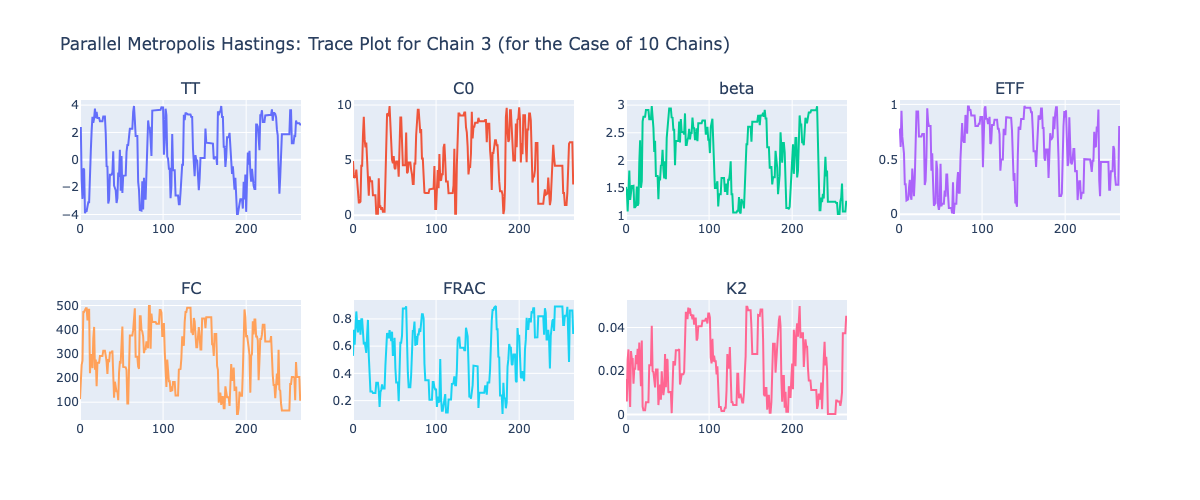
\includegraphics[width=1\textwidth]{figures/parallel_mh/tp_rand_10_3.png}
    \captionsetup{width=.8\textwidth}
    \caption{Trace plot of the third chain from the parallel Metropolis-Hastings algorithm with 10 chains}
    \label{fig:enter-label}
\end{figure}

\begin{figure}[H]
    \centering
    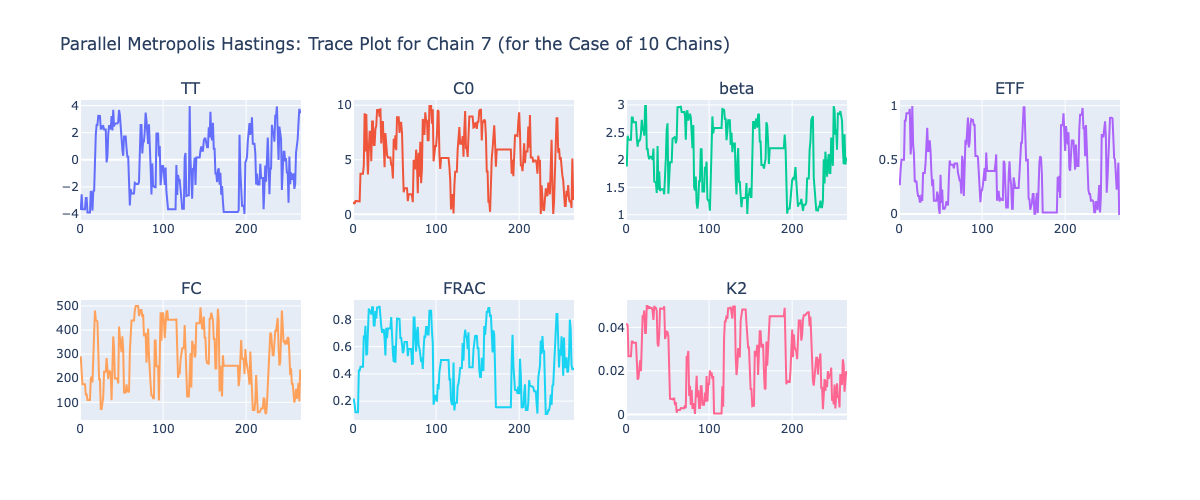
\includegraphics[width=1\textwidth]{figures/parallel_mh/tp_rand_10_7.png}
    \captionsetup{width=.8\textwidth}
    \caption{Trace plot of the seventh chain from the parallel Metropolis-Hastings algorithm with 10 chains}
    \label{fig:enter-label}
\end{figure}

\begin{figure}[H]
    \centering
    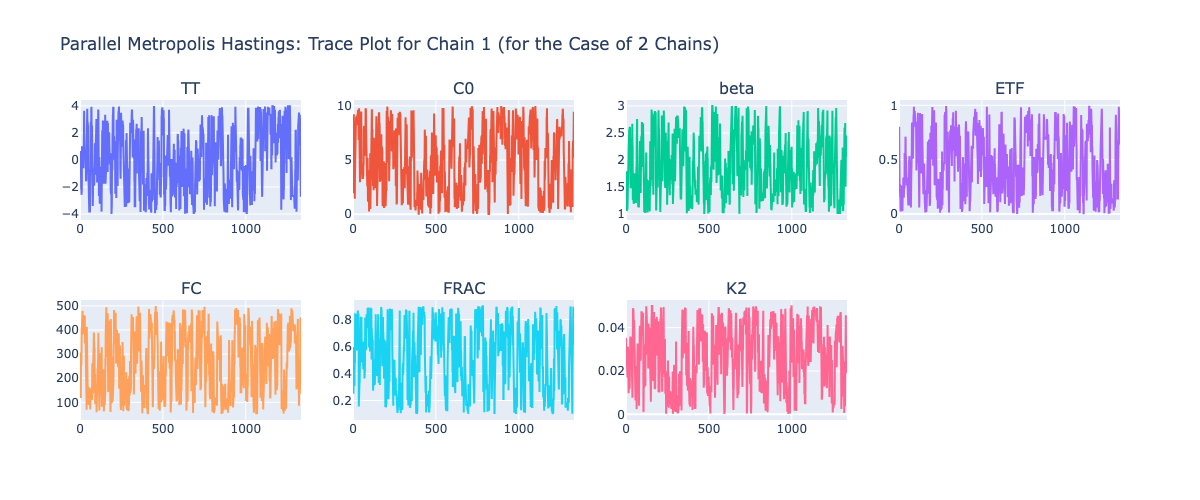
\includegraphics[width=1\textwidth]{figures/parallel_mh/tp_rand_2_1.png}
    \captionsetup{width=.8\textwidth}
    \caption{Trace plot of the first chain from the parallel Metropolis-Hastings algorithm with 2 chains}
    \label{fig:enter-label}
\end{figure}

\begin{figure}[H]
    \centering
    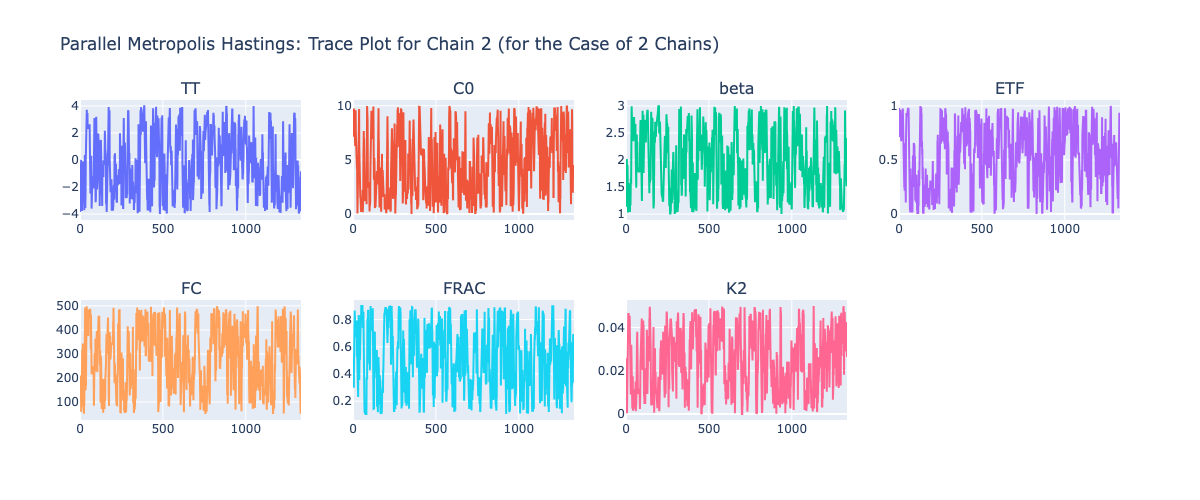
\includegraphics[width=1\textwidth]{figures/parallel_mh/tp_rand_2_2.png}
    \captionsetup{width=.8\textwidth}
    \caption{Trace plot of the second chain from the parallel Metropolis-Hastings algorithm with 2 chains}
    \label{fig:enter-label}
\end{figure}


\section{Gelman Rubin Convergence}
As we mentioned in the introduction of this chapter, the convergence of the result is an aspect that we shall observe after combining all results altogether. This diagnostic helps to determine whether the chains have reached a stationary distribution over time, which shows whether the samples are representative of the target distribution~\cite{gelman_rubin}.

The calculation of Gelman Rubin's diagnostic looks as follows: We define $m$ as the number of chains and $n$ as the number of iterations of each chain. $s_{ij}$ is then the vector of parameters in the $i$th iteration of from the $j$th chain. $\overline{s}_j$ is the mean of vectors within the $j$th chain, whereas $\overline{s}$ is the grand mean vector, calculating the mean of all of the $\overline{s}_j$~\cite{gr_calc}.

\begin{align}
W = \frac 1 {m(n-1)}\sum_{j=1}^m \sum_{i=1}^n (s_{ij} - \overline{s}_j)^2
\end{align}

\begin{align}
B = \frac n {m-1} \sum_{j=1}^m (\overline{s}_j - \overline{s})^2
\end{align}

\begin{align}
V = \frac {n-1}n W + (1 + \frac 1 m)\frac B n
\end{align}

\begin{align}
R = \frac V W
\end{align}

$W$ is called the within-chain variance estimates, which estimate the variances of all sampled points within chains. $B$ is called the average of the between, which measures the variance of the chain means around the overall mean of these means. $V$ is the pooled variance estimate, which is calculated by the weighted versions of $B$ and $W$. Last but not least, the ratio between the pooled an d within chain estimators is calculated and used as the Gelman-Rubin diagnostic. If the diagnostic is close to 1, commonly less than 1.1, it suggests that the chains have converged to the target distribution. A value greater than 1.1 indicates that additional sampling may be necessary, or that the chains have not yet mixed well and may potentially need more iterations~\cite{gr_calc}. For the case of MCMC, the threshold of 1.2 is also tolerated~\cite{gr1.2}.

We now take a look at the performance of Gelman Rubin's convergence in the parallel Metropolis-Hastings algorithm. We take a look at the algorithms with different chain numbers, They are displayed in Figures 5.6 to 5.10. All of these cases show a good enough convergence to show compliance to the threshold of $1.1$, even though a relationship between the convergence level and the number of chains could be found: the more chains there are, the less the result converges.

The reason behind this observation is that each chain generates fewer samples if more chains are used in the parallel Metropolis-Hastings algorithm. In this case, it is more likely that individual chains reach a low level of convergence since it does not generate enough samples. For instance, even though it still satisfies the convergence threshold, the case of $10$ chains shows the worst convergence level of all of the test cases, since it only generates $1000$ samples instead of $2500$ in the case of $4$ chains. Another observation is that no patterns can be found regarding the convergence behavior of individual dimensions. No parameter performs the best or the worst in every single case, which means that further investigation of individual parameters is not needed.

\begin{figure}[H]
    \centering
    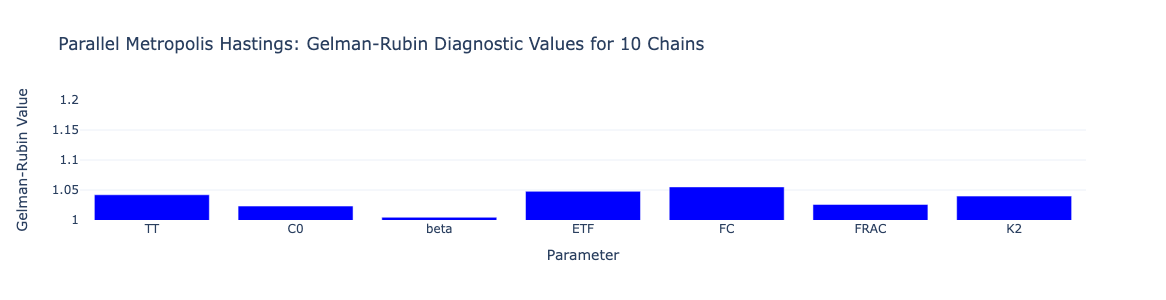
\includegraphics[width=1\textwidth]{figures/parallel_mh/GR_10.png}
    \captionsetup{width=.8\textwidth}
    \caption{Gelman Rubin Convergence Diagnostic of the parallel Metropolis-Hastings algorithm with 10 chains}
    \label{fig:enter-label}
\end{figure}

\begin{figure}[H]
    \centering
    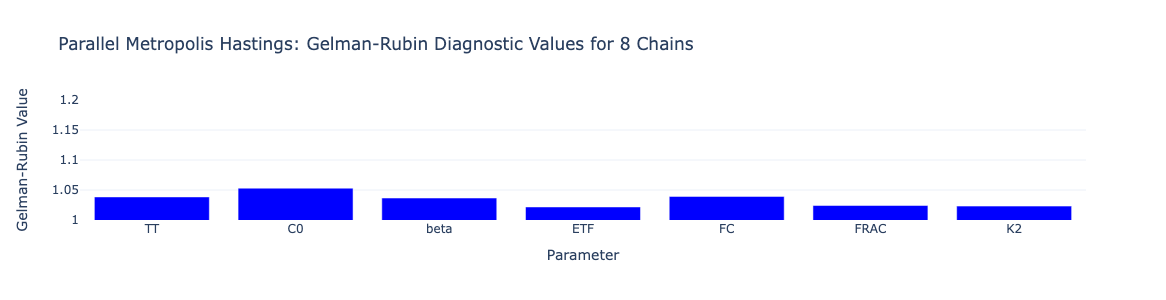
\includegraphics[width=1\textwidth]{figures/parallel_mh/GR_8.png}
    \captionsetup{width=.8\textwidth}
    \caption{Gelman Rubin Convergence Diagnostic of the parallel Metropolis-Hastings algorithm with 8 chains}
    \label{fig:enter-label}
\end{figure}

\begin{figure}[H]
    \centering
    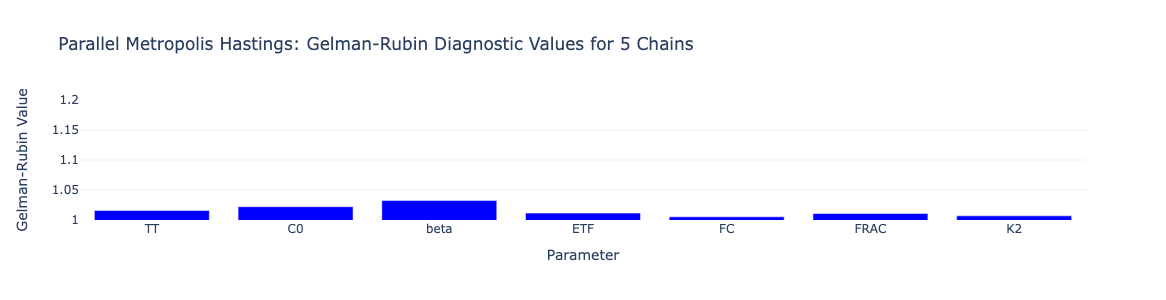
\includegraphics[width=1\textwidth]{figures/parallel_mh/GR_5.png}
    \captionsetup{width=.8\textwidth}
    \caption{Gelman Rubin Convergence Diagnostic of the parallel Metropolis-Hastings algorithm with 5 chains}
    \label{fig:enter-label}
\end{figure}

\begin{figure}[H]
    \centering
    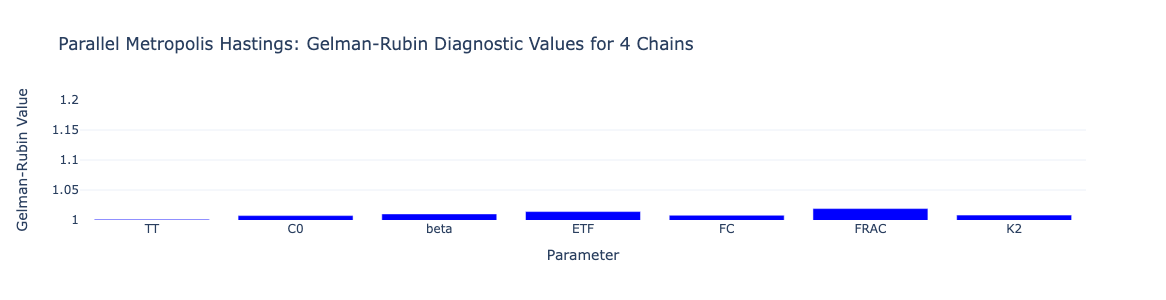
\includegraphics[width=1\textwidth]{figures/parallel_mh/GR_4.png}
    \captionsetup{width=.8\textwidth}
    \caption{Gelman Rubin Convergence Diagnostic of the parallel Metropolis-Hastings algorithm with 4 chains}
    \label{fig:enter-label}
\end{figure}

\begin{figure}[H]
    \centering
    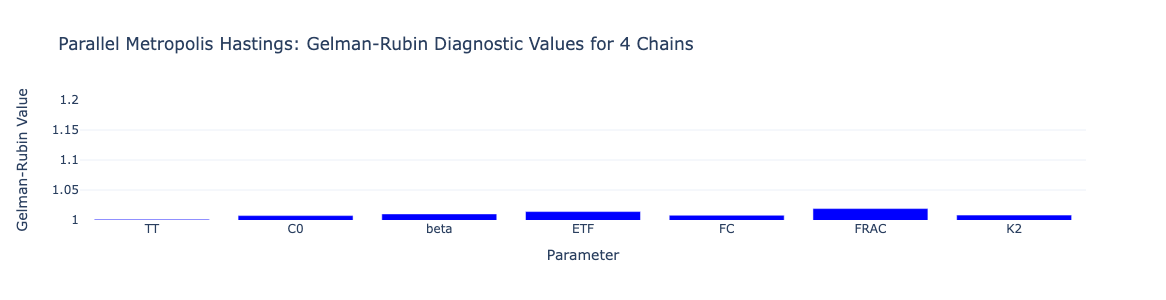
\includegraphics[width=1\textwidth]{figures/parallel_mh/GR_2.png}
    \captionsetup{width=.8\textwidth}
    \caption{Gelman Rubin Convergence Diagnostic of the parallel Metropolis-Hastings algorithm with 2 chains}
    \label{fig:enter-label}
\end{figure}



\section{Autocorrelation Plot}
An autocorrelation plot displays the correlation of a series with itself at different levels of lags. In the context of MCMC, it shows the dependency of the current value in the chain and its past values. This plot is crucial because samples that are generated by Markov chain Monte Carlo algorithms are inherently sequential and may exhibit significant correlation with previous samples, which is something that should be investigated. 

In this section, the autocorrelation of each of the Metropolis-Hastings cases regarding the number of chains is investigated. Since we draw the conclusion from the chapter above that the most optimal effective sample size is $3$, we keep using this number in these test cases.

We first take a look at the cases with the most and the least number of chains, namely $10$ and $2$. These can be found in Figures 5.11 and 5.12. Both autocorrelation graphs share a characteristic that the autocorrelation drops to a low level quickly within a few lags. This suggests that the influence of any given sample on future samples diminishes quickly, which indicates good sampling efficiency. Afterwards, for both cases, the autocorrelation of all dimensions oscillates around 0 and 0.2 positive and negative, which suggests that the sampling shows stability and low correlation to past samples. 

\begin{figure}[H]
    \centering
    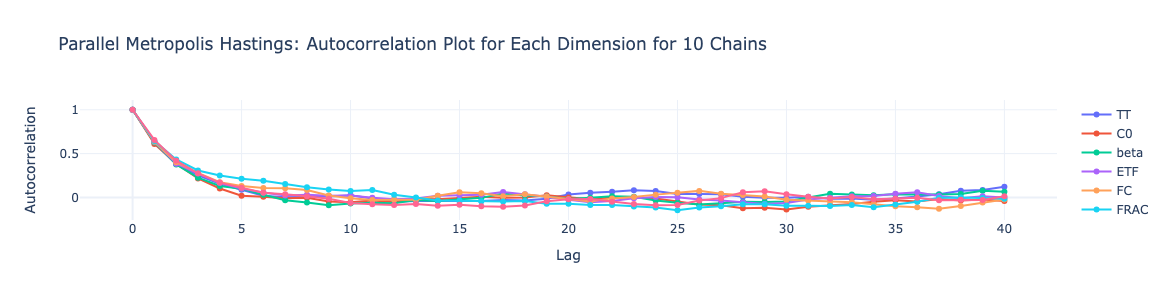
\includegraphics[width=1\textwidth]{figures/parallel_mh/Autocorrelation_10.png}
    \captionsetup{width=.8\textwidth}
    \caption{Autocorrelation plot of the parallel Metropolis-Hastings algorithm with 10 chains}
    \label{fig:enter-label}
\end{figure}


\begin{figure}[H]
    \centering
    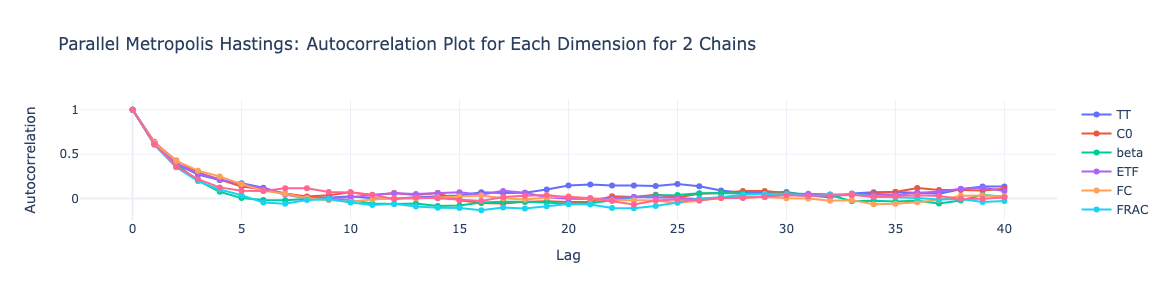
\includegraphics[width=1\textwidth]{figures/parallel_mh/Autocorrelation_2.png}
    \captionsetup{width=.8\textwidth}
    \caption{Autocorrelation plot of the parallel Metropolis-Hastings algorithm with 2 chains}
    \label{fig:enter-label}
\end{figure}


However, both graphs do not display an extremely low level of autocorrelation at high lags. For some parameters, the autocorrelation at high lags approaches $0.2$, which is a relatively high value, even though it is generally acceptable. After plotting graphs for more test cases of the parallel Metropolis-Hastings algorithm using different chains, the autocorrelation graph of the parallel Metropolis-Hastings algorithm using 8 chains delivers a more optimal result. This can be seen in Figure 5.13. Autocorrelations around 20 lags approach closer to zero or show minimal fluctuation around zero. However, the autocorrelation around 40 lags shows a closer distance to 0, which is optimal for the independence property of Markov chain sampling. Nevertheless, all of the other cases of chain numbers show a satisfying result, with rapid diminishing in the first few lags, oscillation around zero, and a relatively low level of autocorrelation for all of the lags apart from the first few.


\begin{figure}[H]
    \centering
    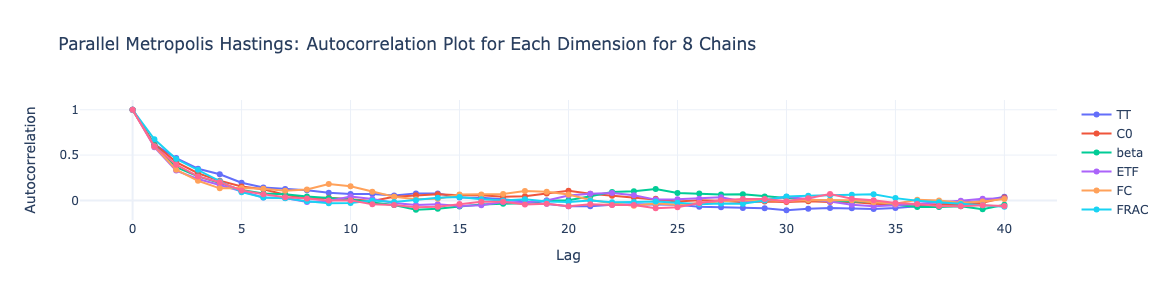
\includegraphics[width=1\textwidth]{figures/parallel_mh/Autocorrelation_8.png}
    \captionsetup{width=.8\textwidth}
    \caption{Autocorrelation plot of the parallel Metropolis-Hastings algorithm with 8 chains}
    \label{fig:enter-label}
\end{figure}


\section{Accuracy Analysis by Chains}
After all these analyses regarding the components of the algorithm, we shall determine the number of chains that suit the algorithm the best. The accuracy metrics are kept the same as the ones that are used in the chapters above the RMSE and MAE. From the graphs shown in Figures 5.14 and 5.15, the parallel Metropolis-Hastings algorithm using 4 chains shows the best level of accuracy in both metrics. Centered around 4, the further the number of chains are, the less accurate they are, however not by a significant difference.

\begin{figure}[H]
    \centering
    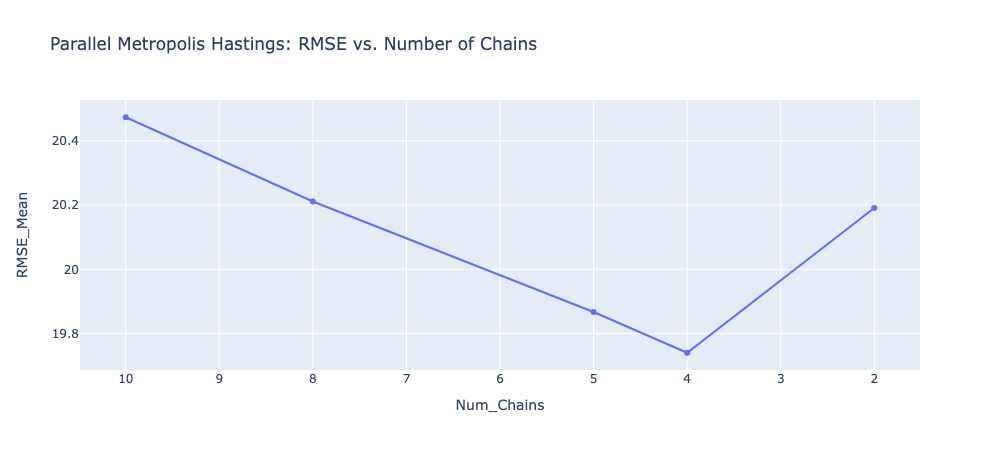
\includegraphics[width=1\textwidth]{figures/parallel_mh/rmse.png}
    \captionsetup{width=.8\textwidth}
    \caption{Mean RMSE of the parallel Metropolis-Hastings algorithm across test cases with different chains}
    \label{fig:enter-label}
\end{figure}

\begin{figure}[H]
    \centering
    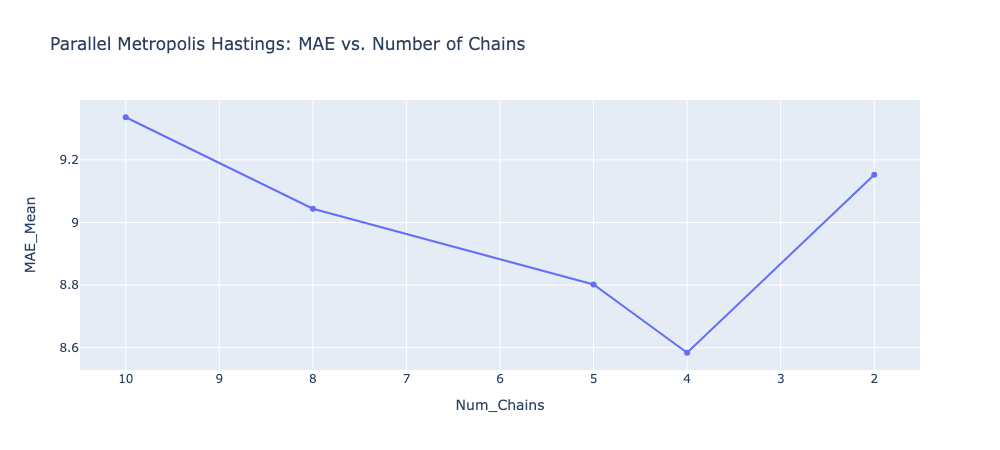
\includegraphics[width=1\textwidth]{figures/parallel_mh/mae.png}
    \captionsetup{width=.8\textwidth}
    \caption{Mean MAE of the parallel Metropolis-Hastings algorithm across test cases with different chains}
    \label{fig:enter-label}
\end{figure}

\section{Parameter Overview}
The last aspect that is focused on in this chapter is the inferred parameter. In the chapter above, we visualized the inferred parameter by visualizing the distribution of the individual parameters. For the case of parallel Metropolis-Hastings, we utilize multiple chains to sample. Therefore, we shall not only just visualize the inferred parameter distribution of the entire result, but also visualize the inferred parameter distribution of each chain and to compare them with the result, to review the stability of the sampling of each chain and also finding out similarities and patterns.

As usual, we first analyze the parameters by a chain for the two extreme cases, namely parallel Metropolis-Hastings with $10$ and with $2$ chains. These can be found in Figures 5.16 and 5.18. From the case of $10$ chains, we can see that the distribution of each chain is relatively random. To compose the distribution of the combined results, each chain is responsible for exploring a different region. For instance, for the parameter TT, the $9$th chain explores the side with lower values more, whereas the $10$th chain is more responsible for the side with higher values. Altogether, this property contributes to the relatively uniform distribution of the combined result. However, there are still similarities to some extent that can be found between the sample distribution of each chain and the sample distribution of the combined result. In each distribution, there are two peaks, each located on the left and the right side of a trough. This means that in each sampling process, two regions can be found that aggregate the most sampling values. Besides, both regions on the left and the right side of the interval acquire fewer samples than other regions, which contribute to the same property of the final combined result. In the case of $2$ chains, things are not so complicated. Because each chain generated more samples than each chain does for the case of $10$ chains, the distribution of each chain looks highly similar to the distribution of the combined result for most of the parameters. For the parameter of ETF, as an exception, it shares the property as the case for $10$ chains, namely that both of the chains are responsible for exploring two different areas, which are the left and the right sides of the entire interval.

Another plot that is used for visualizing the parameters is the boxplot, which is also visualized here in the same way as above: each chain is visualized individually, where they are compared to each other and the combined result boxplot afterward. The figures for cases of $10$ chains and $2$ chains can be found below in Figures 5.17 and 5.19. The results that we can draw from observing these boxplot graphs are the same as the conclusion that we have drawn above for the case of more chains, the $1$st quantile, the median and the $3$ quantile all vary from each other, which means that each chain is responsible for different regions. For the case of fewer chains, however, the $1$st quantile, the median, and the $3$ quantile lie almost on the same level or do not vary from each other that much, indicating that the samples from each chain are more stabilized. 

\begin{figure}[H]
    \centering
    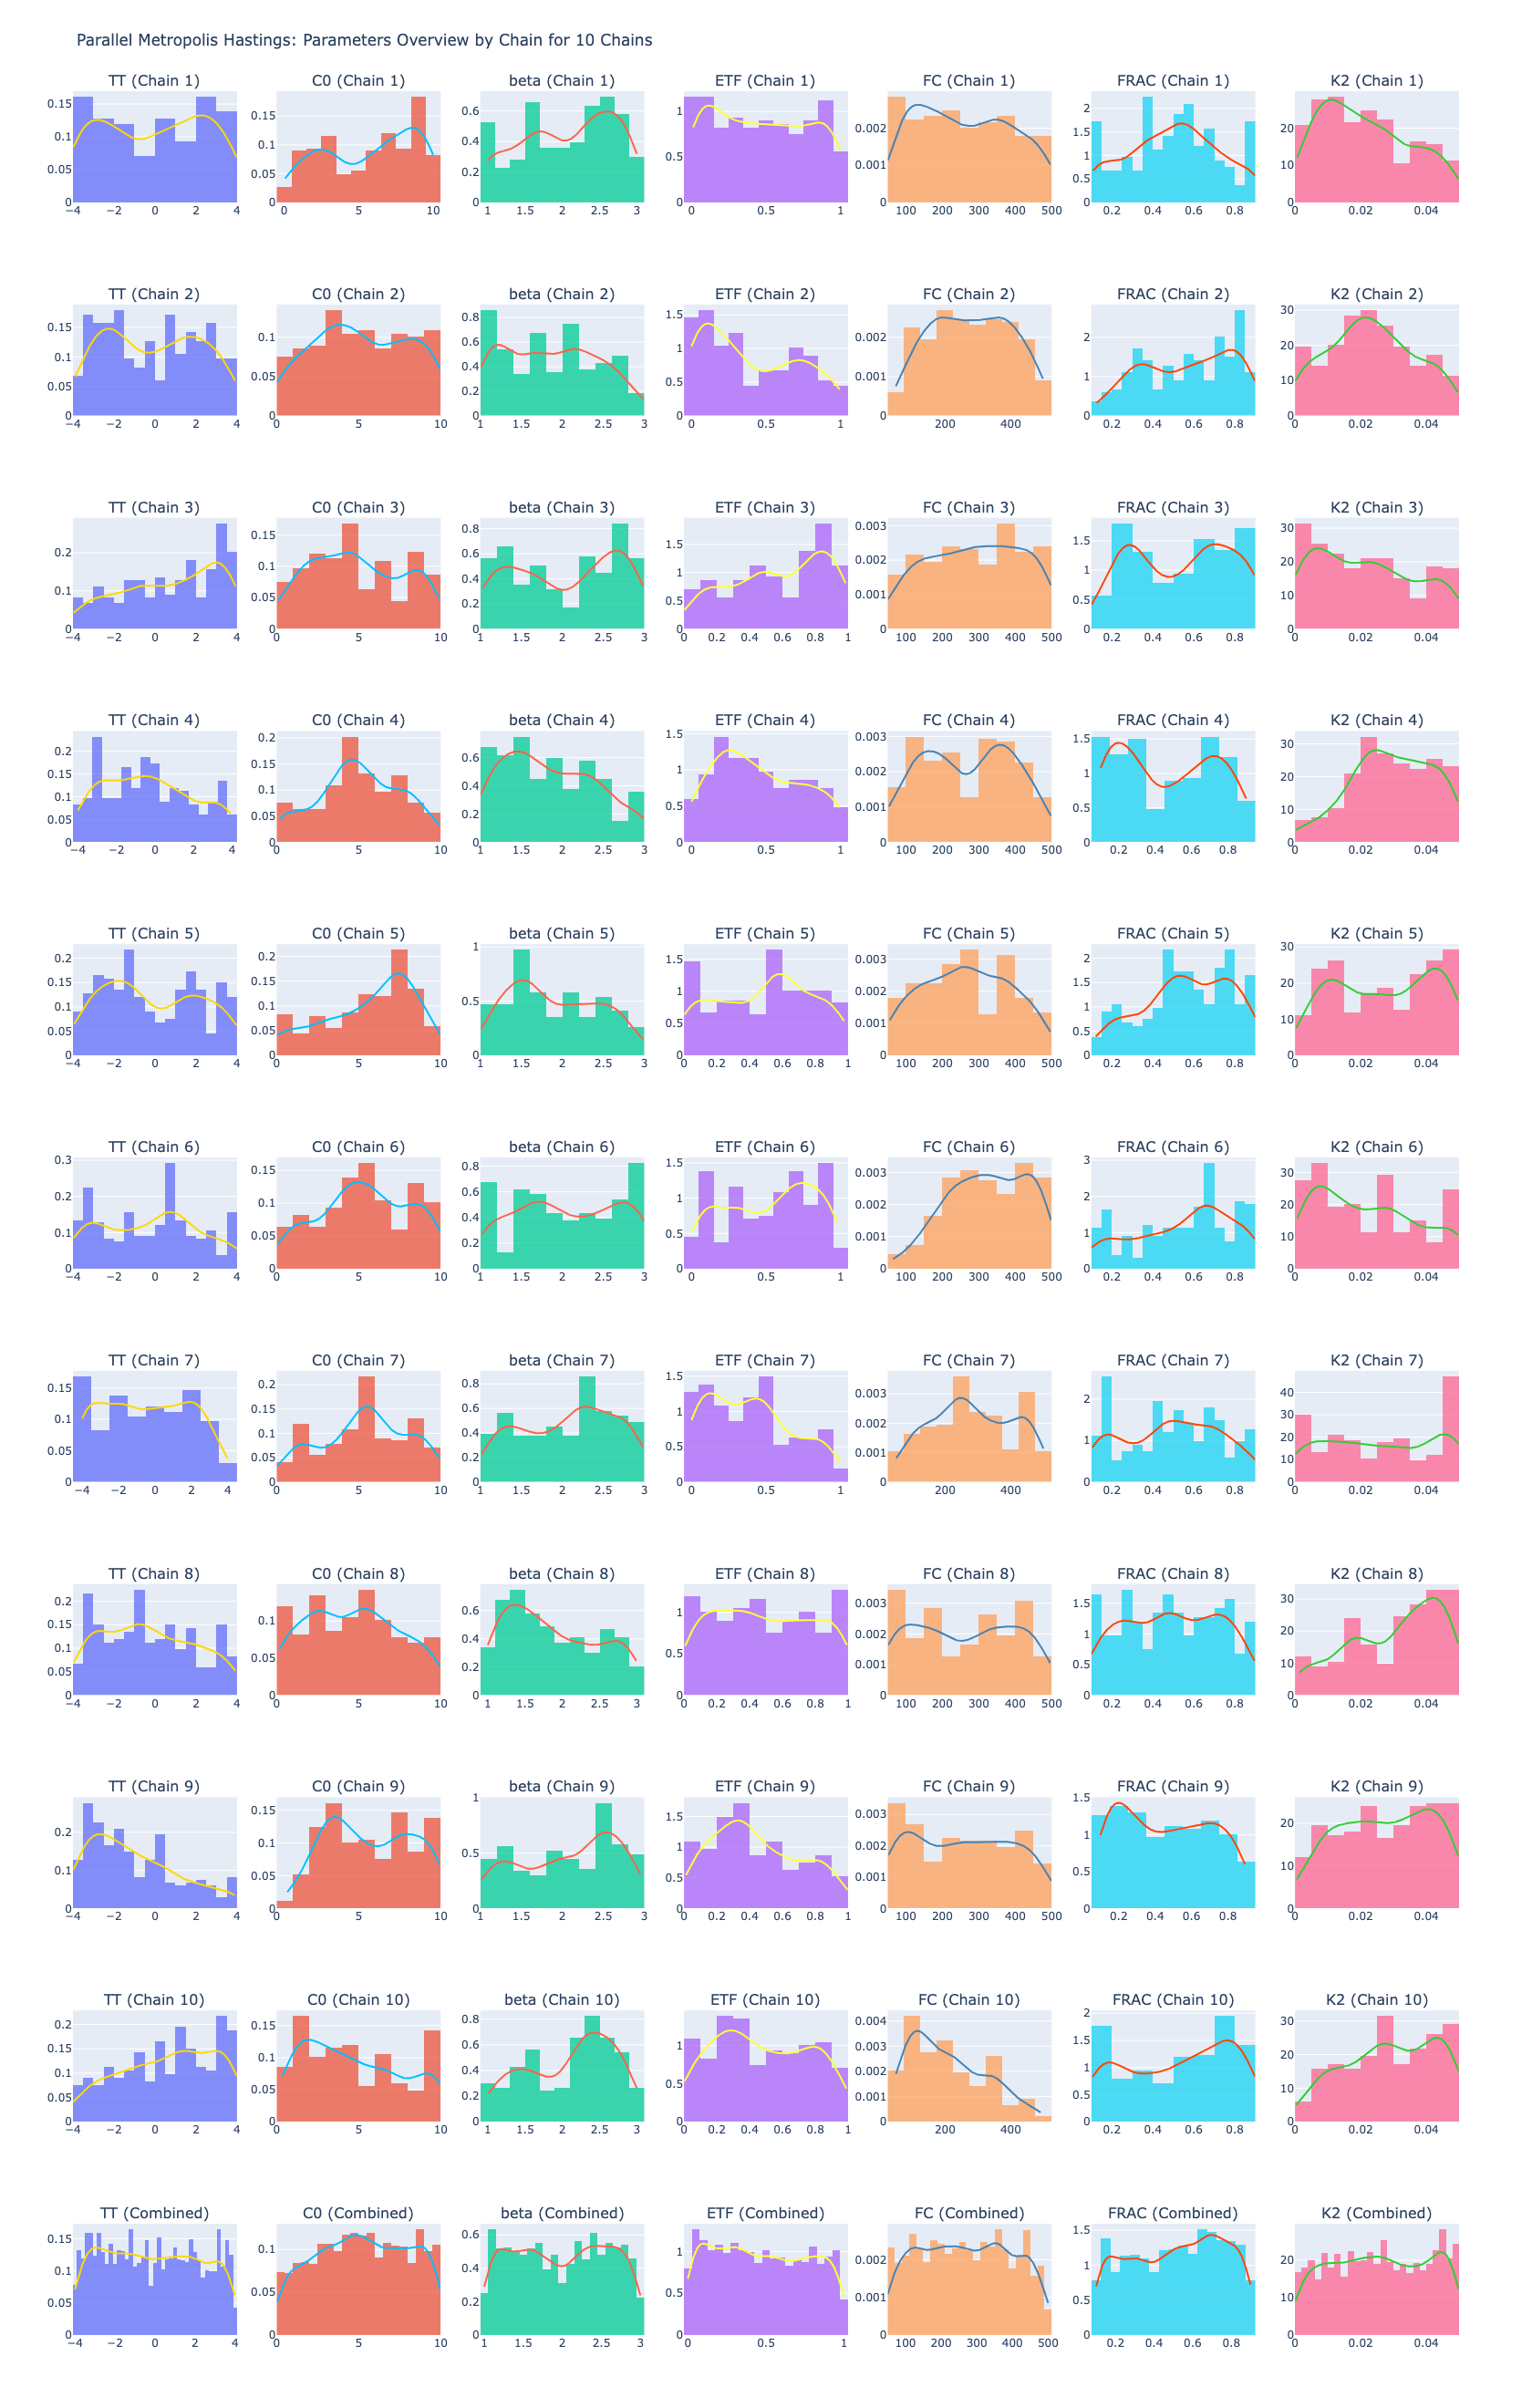
\includegraphics[width=.6\textwidth]{figures/parallel_mh/param_overview_10.png}
    \captionsetup{width=.8\textwidth}
    \caption{Parameter overview by chain for parallel Metropolis-Hastings using 10 chains}
    \label{fig:enter-label}
\end{figure}

\begin{figure}[H]
    \centering
    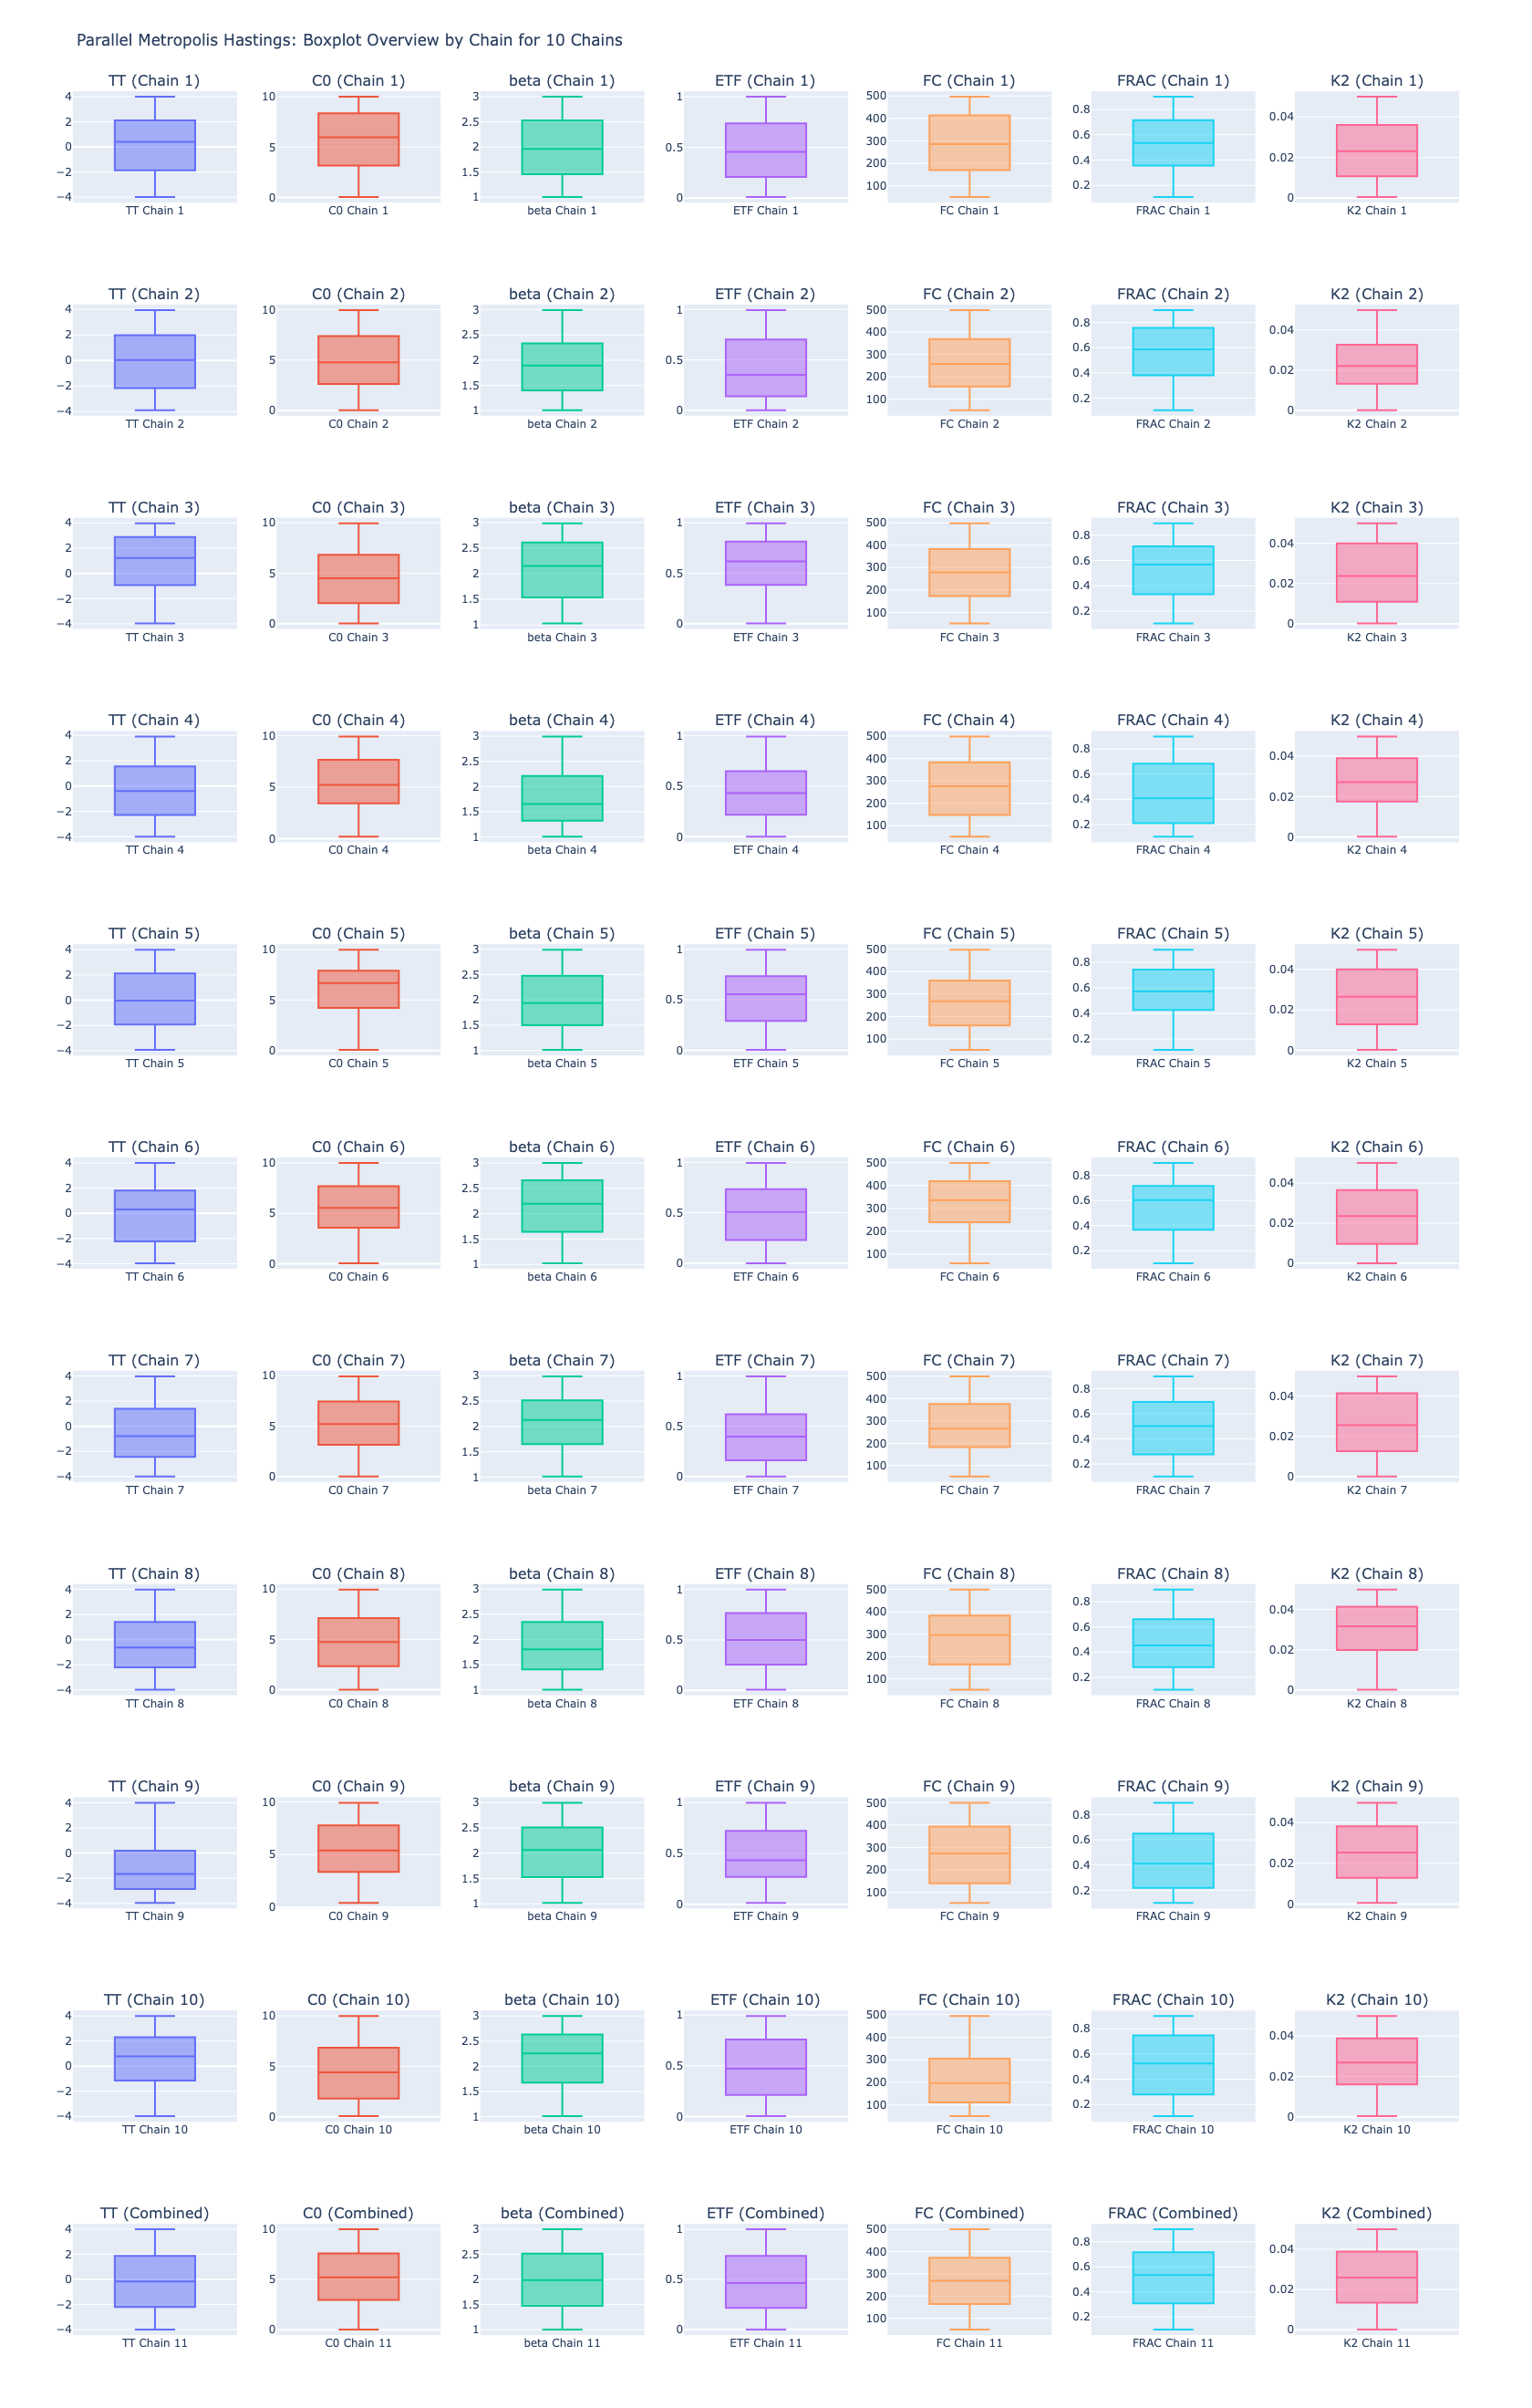
\includegraphics[width=.6\textwidth]{figures/parallel_mh/boxplot_10.png}
    \captionsetup{width=.8\textwidth}
    \caption{Boxplot by chain for parallel Metropolis-Hastings using 10 chains}
    \label{fig:enter-label}
\end{figure}

\begin{figure}[H]
    \centering
    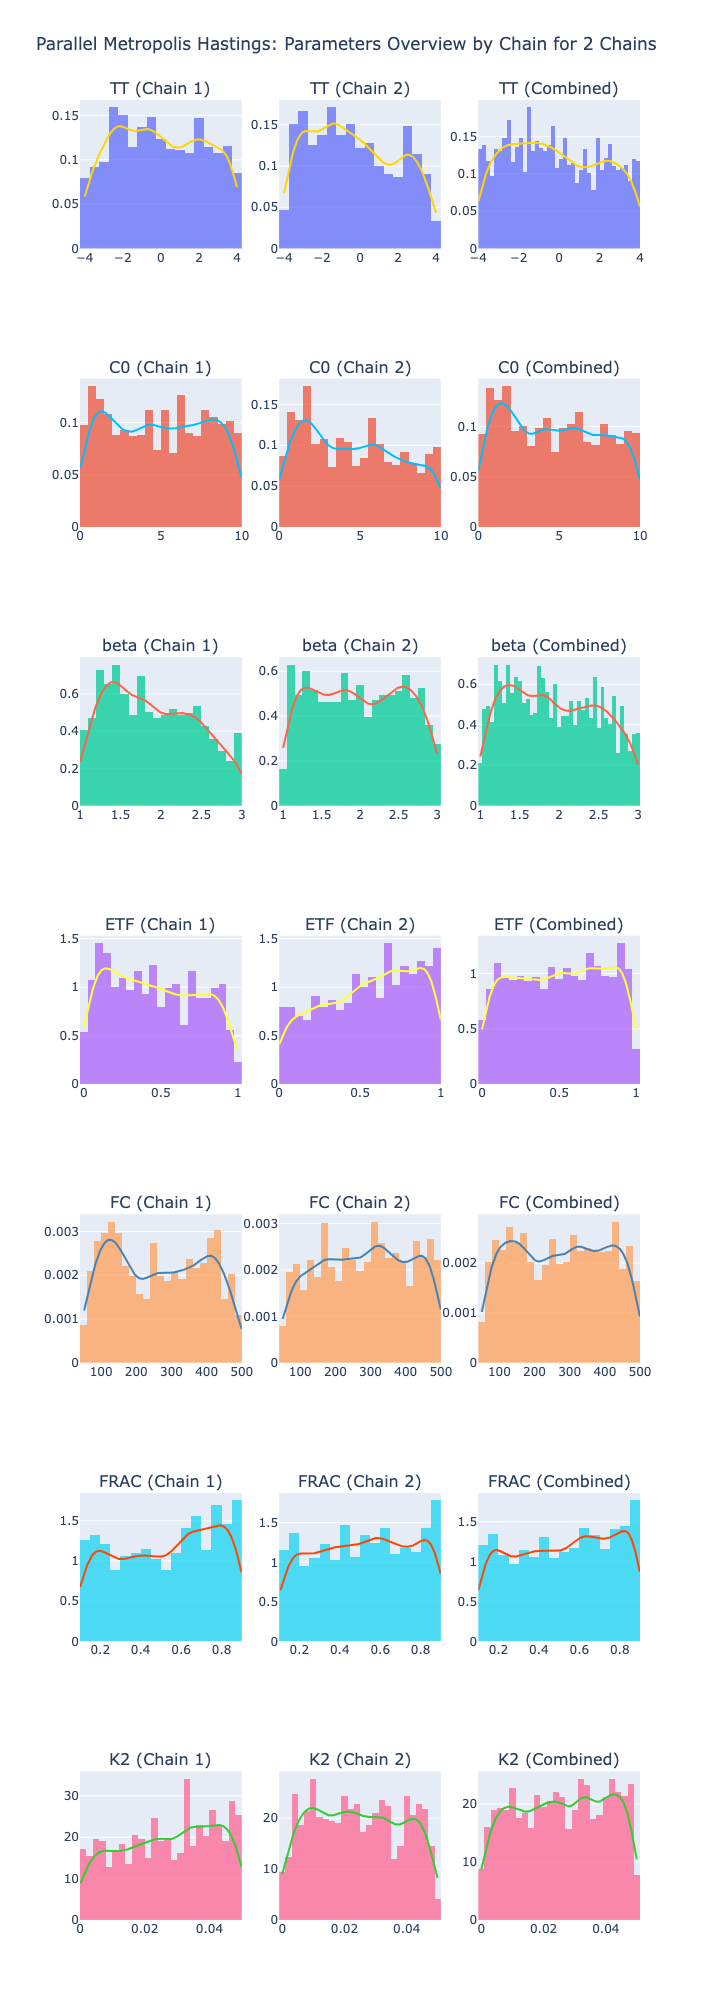
\includegraphics[width=.6\textwidth]{figures/parallel_mh/param_overview_2.png}
    \captionsetup{width=.8\textwidth}
    \caption{Parameter overview by chain for parallel Metropolis-Hastings using 2 chains}
    \label{fig:enter-label}
\end{figure}

\begin{figure}[H]
    \centering
    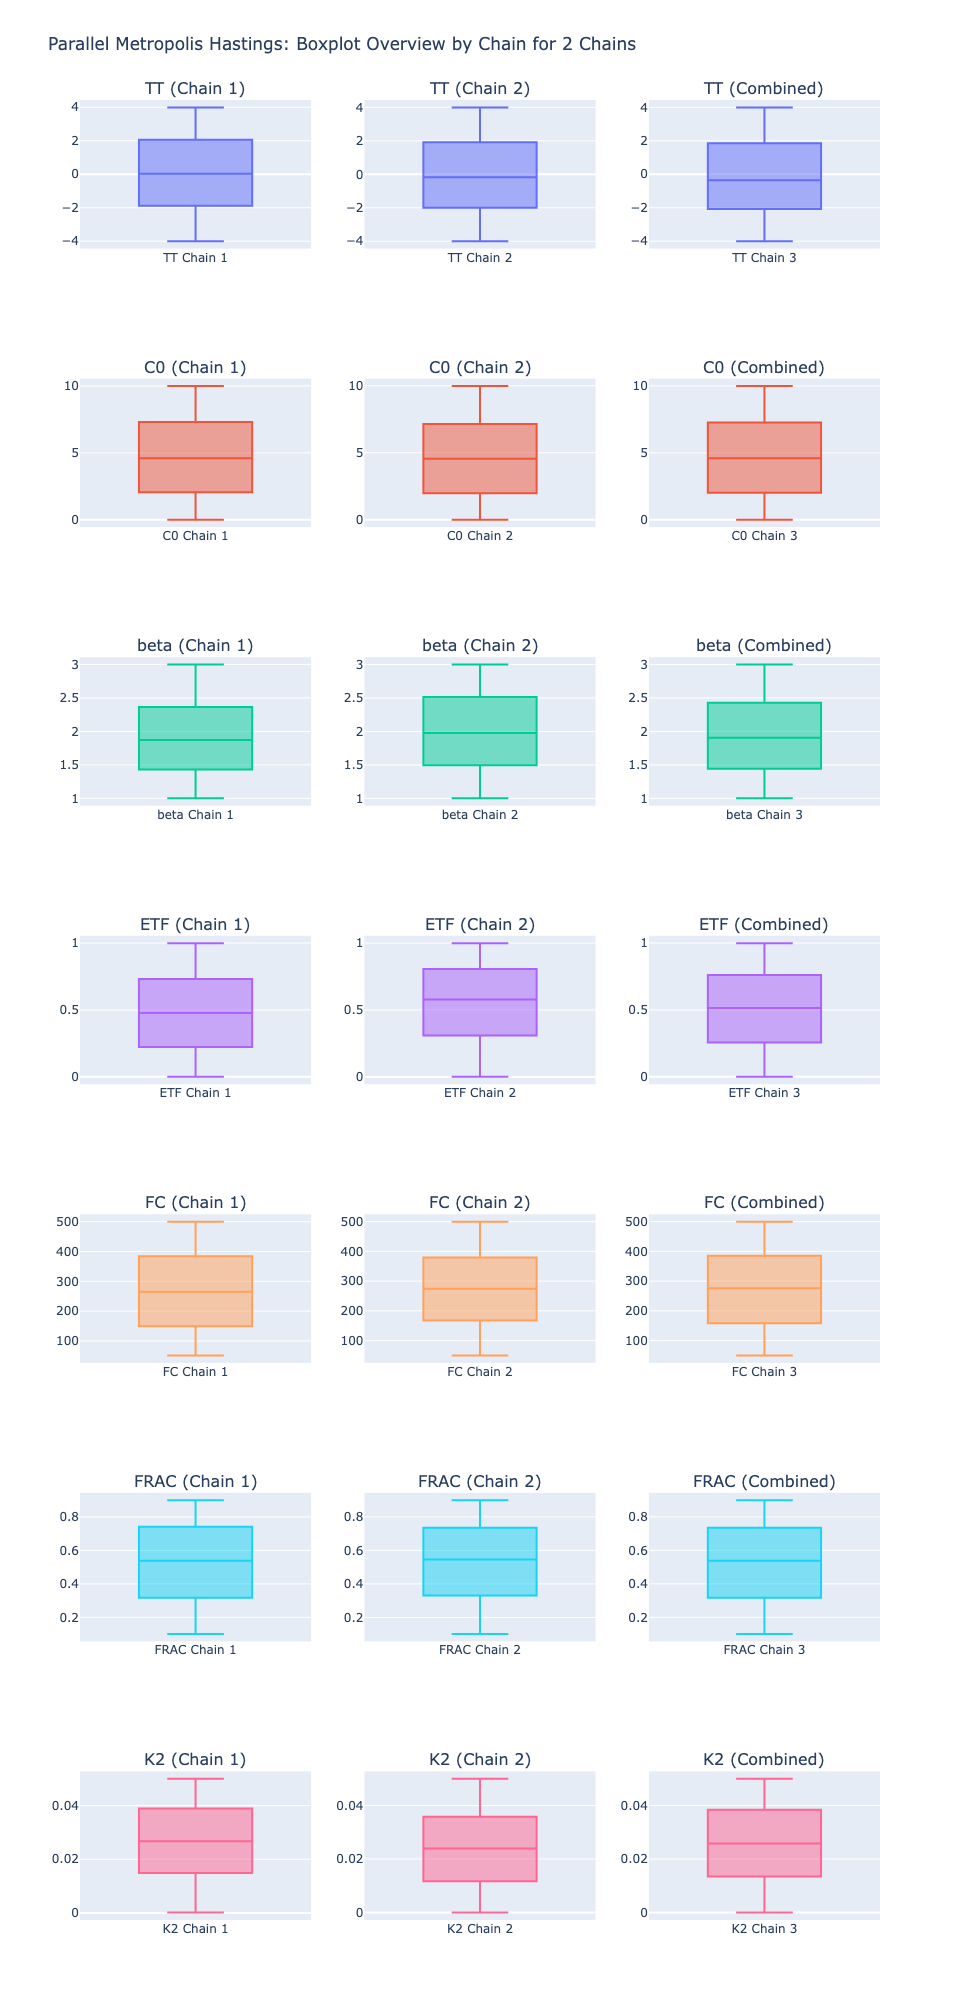
\includegraphics[width=.6\textwidth]{figures/parallel_mh/boxplot_2.png}
    \captionsetup{width=.8\textwidth}
    \caption{Boxplot by chain for parallel Metropolis-Hastings using 2 chains}
    \label{fig:enter-label}
\end{figure}